\chapter{Anexos}



\textbf{Algoritmo}: Un algoritmo se define como un conjunto de ordenes definidas y finitas con el objetivo de llegar a una solución a un problema, la realización de un computo, proceso de datos u otras actividades. El estudio de los algoritmos busca una constante mejora de la resolución de problemas empleando métodos distintos, con el fin de optimizar los recursos necesarios, así como una solución estandarizada y apropiada para un problema general.

\textbf{AI}:

\textbf{API}:

\textbf{Animación}: La animación es el acto de producir imágenes en movimiento; técnica que significa que provee de movimiento a una grabación o una serie de dibujos (Oxford English Dictionary). 

\textbf{Código}: El código en el contexto, se define como el conjunto de símbolos y signos que se transmiten de un emisor a un receptor, cuya intención es privar del conocimiento de su contenido a terceros. Un código tiene un conjunto de reglas o normas que se emplean para dificultar la lectura del mensaje, siendo un ejemplo la traducción de un mensaje en español a ingles, el mensaje puede ser solo entendido por quien conozca el idioma ingles.

\textbf{Cmake}:

\textbf{CUDA}:

\textbf{Dataset}:

\textbf{Decodificador}:

El decodificador es una herramienta que permite descifrar un mensaje codificado. Se refiere a la actividad inversa de la codificación, implica la recepción de un código y de acuerdo al conjunto de normas establecidas para su traducción, se lo interpreta y se obtiene el mensaje inicial que se deseaba recibir.

\textbf{Frame}:
Las grabaciones o serie de dibujos están compuestas por cuadros o Frames en ingles, que son una imagen individual de la secuencia de imágenes que componen la animación para dar la sensación de movimiento. La mayoría de las animaciones emplean de 24 a 30 Frames per second (FPS). 

\textbf{Framework}:

\textbf{Hardware}: El Hardware se entiende como el componente físico de una computadora o dispositivos de Von Neumann. Esta compuesto por el procesador, la tarjeta madre, RAM, disco duro, monitor, dispositivos de entrada y salida, los cuales normalmente se mencionan como componentes y a los dispositivos externos como periféricos\cite{hardwaredef}.

\textbf{GUI}:

\textbf{Interfaz (UI)}: La interfaz puede ser usada tanto en un contexto de Hardware o de usuario, siendo la segunda la definición relevante.
Una interfaz de usuario (UI) tiene la función de otorgar al usuario el control de una aplicación de Software o un dispositivo de Hardware. Uno de los objetivos de la UI es ser amigable con el usuario, permitiendo interactuar con la aplicación de manera intuitiva y natural. Ejemplos de UI pueden ser la pantalla de inicio de una pagina web y de Hardware un control remoto de televisión.

\textbf{Software}:El software esta construido para ejecutar dispositivos von Neumann multiproposito. Un software contienen secuencias de declaraciones de programas abstractos que describen las tareas que deben ser realizadas por una maquina. 

\textbf{Modelo de Von Neumann}: Es una arquitectura de computadoras, su objetivo es explicar como funciona una computadora y la interacción entre sus distintos componentes (CPU, ALU, RAM y otros).

\textbf{Interprete}:El interprete en el contexto informático es un programa traductor que permite ejecutar otros programas a lenguaje máquina, a diferencia de los compiladores, estos solo ejecutan la sección que requieren emplear.


\textbf{Pixel}:



\textbf{Plugin}:

\textbf{Shell}:

\textbf{Script}:

\textbf{SDK}:



\begin{landscape}

\begin{figure}[t!]
	\centering
	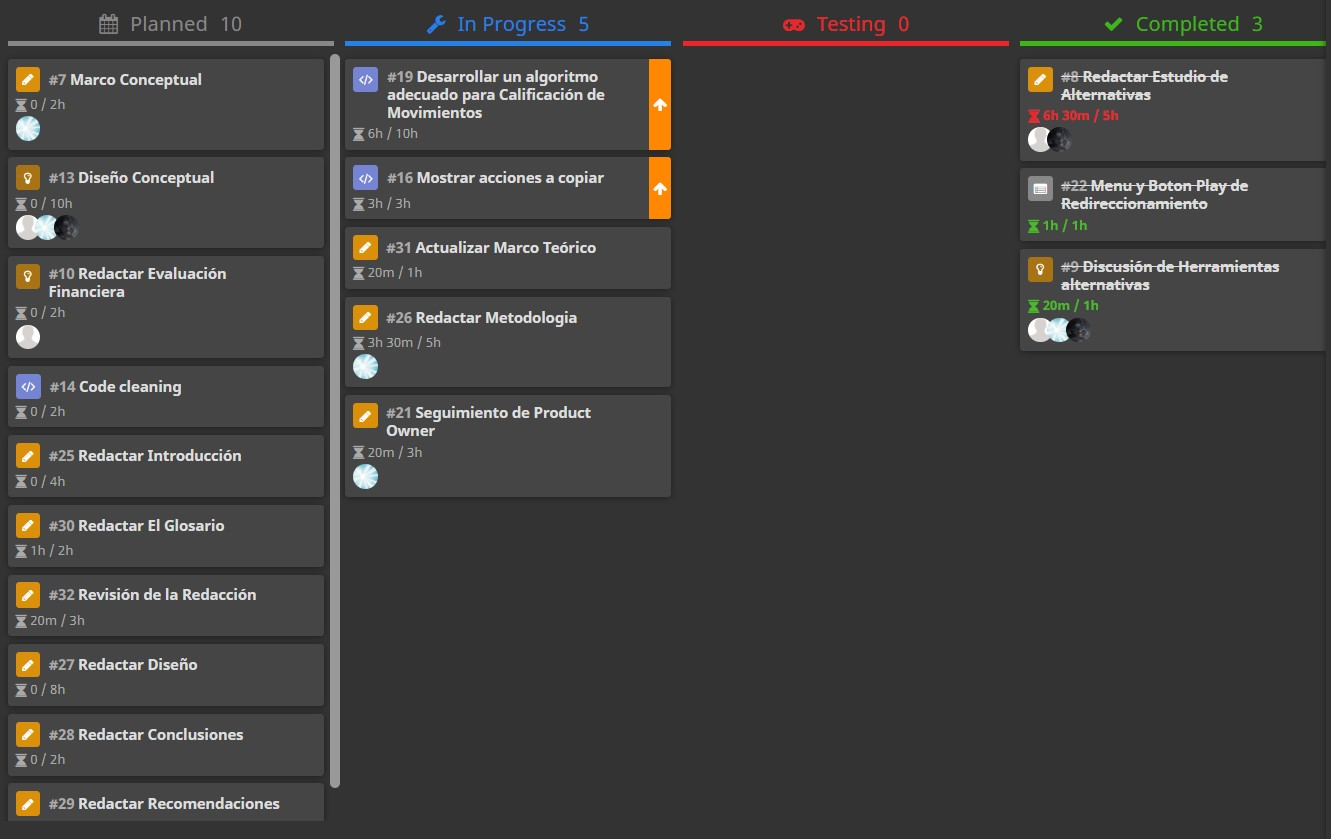
\includegraphics[width=23cm,height=15cm,]{./Images/hacknplanexample.jpg}
	\caption{Sprint Backlog del día 5 de Noviembre}
	\footnotesize Fuente: Elaboración Propia empleando la herramienta HacknPlan.
	\label{sprintexample}
\end{figure}

\end{landscape}
\begin{figure}[t!]
	\centering
	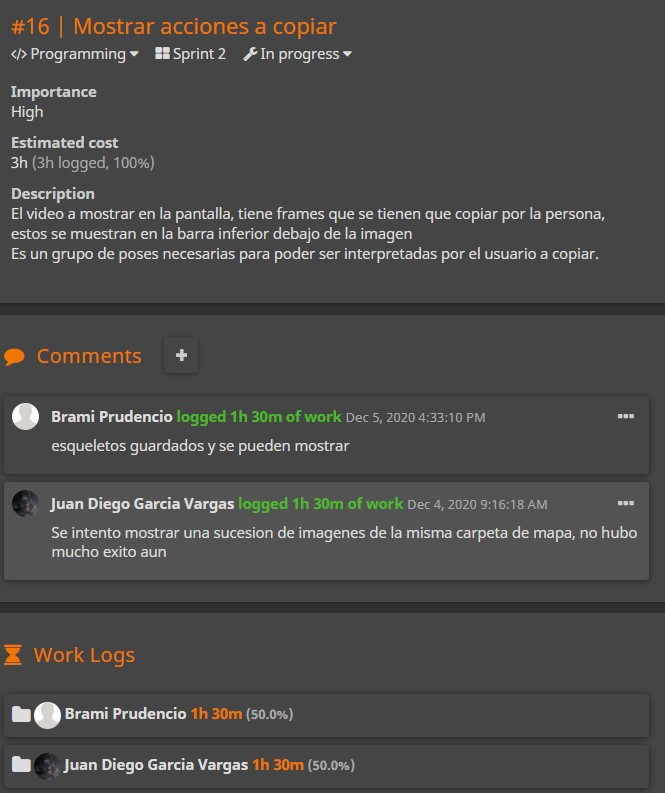
\includegraphics[width=15cm,height=19cm,]{./Images/tareaexample.jpg}
	\caption{Tarea de la Sprint 2, Mostrar Acciones a Copiar}
	\footnotesize Fuente: Elaboración Propia empleando la herramienta HacknPlan.
	\label{sprinttarea}
\end{figure}




